\chapter{3D-модель внешней среды в ostis-системах}
\chapauthortoc{Головатая Е.А.\\Головатый А.И.}
\label{chapter_3D_models}

\vspace{-7\baselineskip}

\begin{SCn}
    \begin{scnrelfromlist}{авторы}
        \scnitem{Головатая Е.А.}
        \scnitem{Головатый А.И.}
    \end{scnrelfromlist}

    \bigskip

    \scntext{аннотация}{Данная глава посвящена рассмотрению вопросов построения и использования трехмерного представления в различных задачах прикладных интеллектуальных систем, а также соответствующих систем позиционирования и ориентации в пространстве. Описание самого представления, а также принципов его построения осуществляется на основе базы знаний ostis-системы, что позволяет проводить глубокую интеграцию различных задач и методов, а также впоследствии приводит к повышению степени конвергенции различных направлений.}

    \bigskip

    \begin{scnrelfromlist}{подраздел}
        \scnitem{\ref{sec_3d_models_problems}~\nameref{sec_3d_models_problems}}
        \scnitem{\ref{sec_3d_models_analysis}~\nameref{sec_3d_models_analysis}}
        \scnitem{\ref{sec_3d_models_approach}~\nameref{sec_3d_models_approach}}
        \scnitem{\ref{sec_3d_models_semantics}~\nameref{sec_3d_models_semantics}}
        \scnitem{\ref{sec_3d_models_representation}~\nameref{sec_3d_models_representation}}
        \scnitem{\ref{sec_3d_models_reconstruction}~\nameref{sec_3d_models_reconstruction}}
        \scnitem{\ref{sec_3d_models_positioning}~\nameref{sec_3d_models_positioning}}
        \scnitem{\ref{sec_3d_models_computervision}~\nameref{sec_3d_models_computervision}}
        \scnitem{\ref{sec_3d_models_actions}~\nameref{sec_3d_models_actions}}
    \end{scnrelfromlist}

    \bigskip

    \begin{scnrelfromlist}{ключевое понятие}
        \scnitem{трехмерное представление объекта}
        \scnitem{трехмерная модель объекта}
        \scnitem{сцена в трехмерном представлении}
        \scnitem{компьютерное зрение}
        \scnitem{оптическая система компьютерного зрения}
        \scnitem{локальный признак изображения}
        \scnitem{трехмерная реконструкция}
    \end{scnrelfromlist}

    \bigskip

    \begin{scnrelfromlist}{библиографическая ссылка}
        \scnitem{\scncite{Berestneva2022}}
        \scnitem{\scncite{Halavataya2019}}
        \scnitem{\scncite{Bay2008}}
        \scnitem{\scncite{Calonder2010}}
        \scnitem{\scncite{Davies2021}}
        \scnitem{\scncite{Halavataya2020}}
        \scnitem{\scncite{Halavataya2022a}}
        \scnitem{\scncite{Halavataya2022b}}
        \scnitem{\scncite{Harris1988}}
        \scnitem{\scncite{Hervas2010}}
        \scnitem{\scncite{Huang2023}}
        \scnitem{\scncite{Krig2016}}
        \scnitem{\scncite{Leutenegger2011}}
        \scnitem{\scncite{Lowe2004}}
        \scnitem{\scncite{Luhmann2018}}
        \scnitem{\scncite{Mair2010}}
        \scnitem{\scncite{Rosten2006}}
        \scnitem{\scncite{Rosten2010}}
        \scnitem{\scncite{Rublee2011}}
        \scnitem{\scncite{Smith1997}}
        \scnitem{\scncite{Verdie2015}}
    \end{scnrelfromlist}

\end{SCn}

\section{Прикладные задачи трехмерной реконструкции}
\label{sec_3d_models_problems}

Для взаимодействия интеллектуальной компьютерной системы с объектами внешней среды в прикладных задачах необходимо создание внутреннего представления этих объектов. Одним из видов такого внутреннего представления может являться описание объектов в виде трехмерной модели. При этом формирование такого внутреннего представления относится к классу задач анализа сенсорной информации и требует определения точного расположения объекта, на основании которого прикладные системы могут реализовывать различные сценарии взаимодействия. В соответствии с этим особую важность приобретают системы ориентации в пространстве и трехмерной реконструкции, способные формировать и обрабатывать такие представления.

К прикладным областям, в которых требуется решение подобных задач, можно отнести \scncite{Luhmann2018}:
\begin{textitemize}
    \item Интеллектуальные робототехнические системы. Примеры задач: анализ окружения, построение траекторий движения, восстановление трехмерных координат объектов.
    \item Интеллектуальные системы управления производством.  Примеры задач: анализ деформаций объектов и структурных изменений, бесконтактное измерение размеров объектов произвольного масштаба и конфигурации, контроль производственного процесса.
    \item Интеллектуальные системы комплексного медицинского мониторинга и обслуживания. Примеры задач: анализ результатов обследований, отслеживание динамики развития заболеваний, планирование лечения.
    \item Научно-исследовательская деятельность.
    \item Другие прикладные области (архитектура, картография и т.д.).
\end{textitemize}

Предметная область трехмерного представления объектов затрагивает, как само описание объекта, так и методов его получения. На основании данных представлений могут быть решены следующие классы задач:

\begin{textitemize}
    \item построение трехмерного представления объекта, группы объектов или окружения,
    \item определение размеров объекта, включающее и определение отклонений от заданного шаблона или параметров, например, в системах медицинской диагностики,
    \item проведение дополнительных построений, доопределяющих созданное сформированное трехмерное представление,
    \item построение траектории движения,
    \item и т. д.
\end{textitemize}

Несмотря на то, что часть указанных выше задач требует дополнительных действий, все они основываются на получении трехмерного представления объекта.

Таким образом, декларативной формулировкой задачи трехмерной реконструкции является получение внутреннего представления объекта, относящегося к классу трехмерных представлений.

\section{Анализ существующих подходов к трехмерной реконструкции}
\label{sec_3d_models_analysis}

На данный момент существует большое количество методов реконструкции, оперирующих разными представлениями входных данных и информации: фотограмметрическое восстановление по фото/видеосъемке, радиочастотные методы в разных диапазонах, магнитные и инерциальные методы, нейросетевой анализ и т.д. Например, искусственные нейронные сети, решающие задачу трехмерной реконструкции, могут принимать в качестве входного значения отдельные изображения, наборы изображений, панорамные и стереоскопические изображения, комбинацию изображений и данных с различных видов датчиков, наборы ключевых точек, воксельное облако. Для каждого метода может быть определен набор характеристик внешней среды (помещение, освещение, наличие движения) и входного представления (размер, тип поверхности), в пределах которых данный метод является корректным и демонстрирует наилучшие результаты работы по одному из целевых критериев. Полученное внутреннее представление также может отличаться: часть методов позволяет восстановить внутреннюю структуру, другие - только поверхность (внешнюю форму) объекта.

Кроме этого в задачах анализа сенсорной информации, как правило, есть возможность установить несколько разных типов датчиков, но они должны быть, во-первых, пригодны для исследования данного типа объекта, а, во-вторых, полученная информация должна дополнять друг друга (увеличивать детализацию модели, разрешающую способность, точность и т.д.), то есть система должна иметь возможность адаптироваться под конкретную задачу и внешние условия.

Все эти факторы накладывают серьзеные ограничения на возможность применения различных методов трехмерной реконструкции при решении конкретной прикладной задачи, которые должны быть учтены при проектировании системы (см. \scncite{Halavataya2022b}).

К проблемам существующих решений можно отнести:
\begin{textitemize}
    \item Отсутствие согласованности систем понятий и описаний методов в различных источниках. Встречаются разные описания одного и того же метода, существует много модификаций, постоянно возникают сложности и, как минимум, недопонимания в связи с этим.
    \item Отсутствие привязки и недостаточное внимание вопросам конвергенции предметной области трехмерной реконструкции с преметной областью формирования трехмерных сцен и окружений интерактивного пользовательского взаимодействия с трехмерной средой, например, в системах трехмерного моделирования, виртуальной и дополненной реальности.
    \item Высокая сложность разработки прикладных систем, использующих методы трехмерной реконструкции, и необходимость привлечения опытных высококвалифицированных разработчиков к решению соответствующих задач.
    \item Отсутствие комплексной технологии проектирования. Несмотря на обилие алгоритмов и методов, анализ их применимости к различным видам прикладных задач крайне поверхностный. Вследствие этого в большинстве случаев лучший метод выбирается перебором или эмпирически.
    \item Отсутствие средств интеграции отдельных компонентов, этапов различных методов, различного типа данных при описании объекта и полученных внутренних представлений. Кроме вариативности отдельных действий, в результате каждый метод работает со своим классом внутреннего представления (поверхность, заданная полигонально, воксельное облако с регулярной сеткой, набор отдельных координат в трехмерном пространстве и т.д.).
\end{textitemize}

Таким образом, систематизация знаний данной предметной области, а также создание технологии разработки и автоматизации процесса проектирования интеллектуальных систем в данной области являются актуальными и нерешенными на данный момент задачами.

\section{Предлагаемый подход к трехмерной реконструкции с использованием базы знаний ostis-системы}
\label{sec_3d_models_approach}

Описание самого представления, а также принципов его построения осуществляется в виде базы знаний ostis-системы. В рамках формирования базы знаний и платформы для разработки интеллектуальных систем в данной предметной области должны быть решены следующие задачи:

\begin{textitemize}
    \item выделение семантического представления трехмерных сцен;
    \item систематизация предметной области, существующих подходов и установление связей со смежными областями;
    \item разработка набора агентов, определяющих подходящие методы и средства для конкретных прикладных задач;
    \item разработка набора агентов, проводящих агрегацию разных методов, с целью уточнения или проверки параметров трехмерного представления (положения) объекта.
\end{textitemize}

Последовательность основных этапов процесса трехмерной реконструкции и их связь с базой знаний OSTIS представлена на рисунке \textit{\nameref{fig:schema-3d-reconstruction}}. В рамках базы знаний ostis-системы трехмерного представления объектов выделены следующие блоки и взаимосвязи:

\begin{textitemize}
    \item описание характеристик наблюдаемых объектов;
    \item описание типов и принципов задания трехмерных представлений;
    \item описание физических принципов работы и спецификаций оборудования, с помощью которого может быть собрана информация об исследуемом объекте;
    \item набор различных методов реконструкции и локализации с ограничениями и решателями конкретных задач;
    \item методы оценки результатов полученных 3D-представлений;
    \item описание семантического представления трехмерных сцен и объектов.
\end{textitemize}

\begin{figure}[H]
    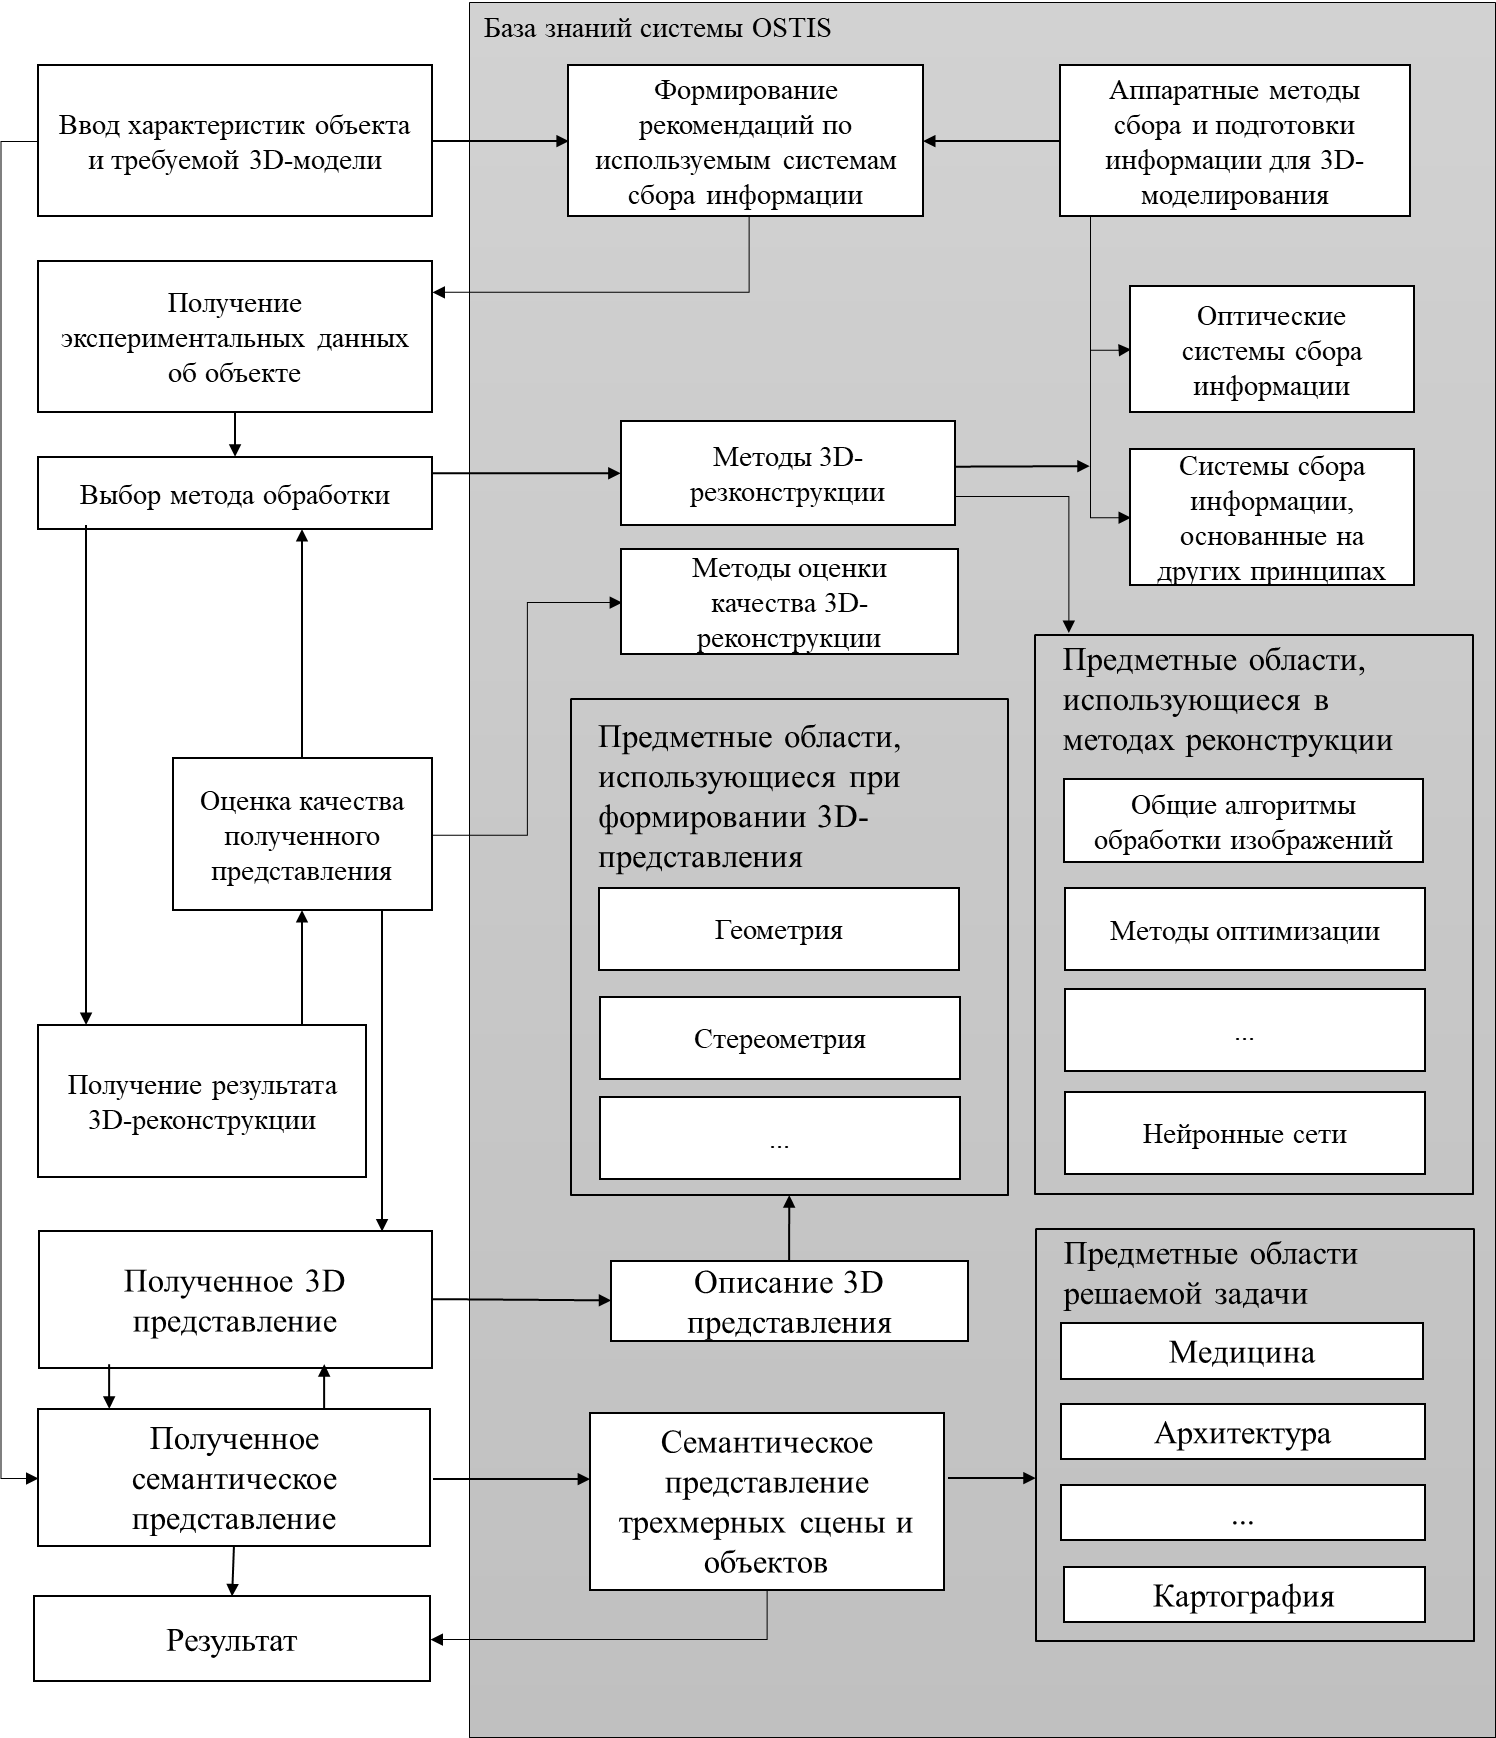
\includegraphics[scale=0.3]{author/part4/figures/schema3D.png}
    \caption{Описание основных этапов процесса трехмерной реконструкции и их связи с базой знаний ostis-системы трехмерного представления объектов}
    \label{fig:schema-3d-reconstruction}
\end{figure}

Далее более подробно рассмотрим основные указанные предметные области и онтологии.

\section{Семантическое представление объектов и сцены}
\label{sec_3d_models_semantics}

Важной составляющей интеллектуальных систем, использующих внутреннее трехмерное представление, является описание семантики этого представления. Информация об индивидуальных точках, поверхностях, полигонах или других примитивах не позволяет сформировать комплексное представление о смысловом наполнении этого представления -- точно так же, как отдельные буквы не позволяют оценить семантическую составляющую текстовых сообщений. Ostis-система предоставляет возможность формирования связанного семантического представления объекта, использующего дополнительную информацию из предметной области рассматриваемого объекта.

В работе \scncite{Huang2023} продемонстрирована возможность использования такого комбинированного представления в задачах машинного обучения и распознавания образов. Данное представление также является основой для задач создания контента, в том числе основанных на генеративных состязательных нейросетевых моделях. Кроме этого, сопоставление пространственных и семантических свойств объекта способствует расширению функциональности и точности человеко-машинного взаимодействия в системах дополненной и виртуальной реальности, например, при проектировании обучающих или вспомогательных приложений (см. \scncite{Berestneva2022}, \scncite{Hervas2010}).

Семантическое описание объекта подразумевает ассоциацию множества точек, соответствующего некоторому объекту в трехмерном пространстве, с некоторым объектом имеющейся базы знаний. Отношения в таких ассоциациях могут быть представлены в виде ``объект А представляет собой трехмерный образ некоторой сущности В'', где объект А задаётся внутренним трехмерным представлением, а сущность В -- некоторым описанием в базе знаний.

Некоторые свойства сущности В, ассоциируемой с объектом А, могут быть естественным образом выведены из трехмерного представления этого объекта -- в частности, информация о форме, свойствах поверхности, окраске и текстурировании могут уже присутствовать в трехмерном описании. Таким образом, с помощью дополнительной обработки трехмерное представление объекта А может являться источником фактологической информации о связанной сущности В. В то же время знание свойств сущности B может помочь при формировании более точного трехмерного образа объекта A. 

Аналогично семантическому описанию отдельного объекта может быть введено семантическое описание составных объектов. Следует иметь в виду, что семантическое наполнение индивидуальных составляющих не позволяет в полной мере определить семантику всего составного объекта целиком, поэтому аналогичную ассоциацию также необходимо задать и для всей совокупности. Например, объект ``велосипед'' может быть декомпозирован на составные объекты ``цепь'', ``рама'', ``колесо'' и т.д., однако набор семантических описаний трехмерных представлений составляющих по отдельности не позволяет формировать или учитывать семантику всего составного объекта целиком.

Семантическое описание части объекта должно содержать как информацию о базовом объекте, так и о дополнительном контексте относительно смыслового наполнения рассматриваемой части. Например, при видеоэндоскопическом анализе участка пищевода важной становится также информация о том, к какой именно части пищевода в организме относится этот участок.

Сцена представляет собой сложную композицию нескольких простых или составных объектов в некотором общем пространстве, дополненную данными об их взаимном расположении. Как и в случае с составными объектами, семантическое описание сцен должно включать не только описания индивидуальных составляющих, но и также смысловое наполнение эмержентных свойств всех этих составляющих в совокупности.

Таким образом, выделены следующие виды основных сущностей в рамках семантического представления сцен и объектов в трехмерном представлении:

\begin{SCn}
    \scnheader{объект в трехмерном представлении}
    \scnidtf{множество точек в пространстве, соединенных между собой и имеющих одно смысловое представление}
\end{SCn}
\begin{SCn}
    \scnheader{составной объект в трехмерном представлении}
    \scnidtf{объект в трехмерном представлении, подразумевающий декомпозицию на отдельные индивидуальные объекты}
\end{SCn}
\begin{SCn}
    \scnheader{часть объекта в трехмерном представлении}
    \scnidtf{множество точек в пространстве, принадлежащих некоторому объекту в трехмерном представлении, которое может быть выделено по его геометрическому или смысловому представлению}
\end{SCn}
\begin{SCn}
    \scnheader{сцена в трехмерном представлении}
    \scnidtf{совокупность нескольких объектов в трехмерном представлении и данных об их взаимном расположении в пространстве и свойствах, включающих абсолютные и относительные референтные ориентированные и неориентированные отношения}
\end{SCn}

Для сцены в трехмерном представлении важными являются семантические характеристики визуального восприятия сцены с позиции некоторого помещенного в неё наблюдателя или системы машинного зрения. В этом контексте сцена может быть представлена в виде отдельного наблюдения, например, двумерной проекции (или пары двумерных проекций в случае стереоскопического зрения). При этом семантика описаний исходных объектов в трехмерном представлении и соответствующих им участков полученных проекций также может отличаться -- например, некоторые объекты могут находиться вне поля видимости, или восприниматься наблюдателем по-другому из-за наличия внешних факторов. К внешним факторам можно отнести наличие оптических, перспективных или психофизиологических эффектов (например, разница в освещении, оптическая дисторсия, различные иллюзии восприятия цвета или глубины, например, комната Эймса, и т.п.). 

Таким образом, важным является тот факт, что семантическое описание сцены должно включать как определение принадлежности индивидуальных объектов сцены некоторым сущностям имеющейся базы знаний, так и описание возможных взаимосвязей между этими объектами, возникающих в силу их присутствия в сцене, или в силу их попарного взаимного расположения с позиции некоторого наблюдателя. Эта информация может естественным образом использоваться в качестве референтных свойств объектов сцены. Например, при наличии в сцене двух одинаковых объектов типа А и одного объекта типа В, некоторое логическое высказывание или запрос на естественном языке может использовать факт их взаимного расположения, например, для идентификации -- ``тот объект типа А, который находится слева от объекта типа Б''.


\begin{SCn}
    \scnheader{внешний фактор наблюдения сцены в трехмерном представлении}
    \scnidtf{параметр наблюдения сцены в трехмерном представлении, определяющий пространственные, психофизические, визуальные и другие свойства восприятия системы наблюдения}
\end{SCn}
\begin{SCn}
    \scnheader{наблюдение сцены в трехмерном представлении}
    \scnidtf{описание сцены в трехмерном представлении при фиксированном состоянии одного или нескольких параметров наблюдения, может заключаться в понижении размерности представления информации, например, при приведении к двумерной проекции}
\end{SCn}
\begin{SCn}
    \scnheader{референтное отношение описания сцены в трехмерном представлении}
    \scnidtf{абсолютные и относительные ориентированные и неориентированные отношения отдельного наблюдения сцены в трехмерном представлении}
\end{SCn}


Ниже приведены некоторые возможные референтные отношения описания сцены в трехмерном представлении относительно различных внешних факторов наблюдения. Следует отметить также, что в общем случае внешний фактор наблюдения может быть задан произвольно соответстветствующей оценочной функцией, например, определения "схожести"{} объектов.

\begin{textitemize}
    \item Информация о присутствии на сцене или проекции сцены
    \begin{textitemize}
        \item Объект отсутствует на сцене
        \item Объект присутствует, но не виден на проекции
        \item Объект присутствует и на проекции виден частично
        \item Объект присутствует и на проекции виден полностью
    \end{textitemize}
    \item Информация о взаимном расположении на проекции сцены
    \begin{textitemize}
        \item По глубине
        \begin{textitemize}
            \item За другим объектом
            \item Перед другим объектом
        \end{textitemize}
    \end{textitemize}
    \begin{textitemize}
        \item По высоте
        \begin{textitemize}
            \item Выше другого объекта
            \item На одном уровне с другим объектом
            \item Ниже другого объекта
        \end{textitemize}
    \end{textitemize}
    \begin{textitemize}
        \item По расположению вдоль линии горизонта
        \begin{textitemize}
            \item Слева от другого объекта
            \item Справа от другого объекта
        \end{textitemize}
    \end{textitemize}
    \item Информация об относительном размере объектов на проекции
    \begin{textitemize}
        \item Больше другого объекта
        \item Одного размера с другим объектом
        \item Меньше другого объекта
    \end{textitemize}
    \item Информация о визуальном сходстве объектов
    \begin{textitemize}
        \item Похож или не похож на другой объект по форме
        \item Похож или не похож на другой объект по цвету
        \item Похож или не похож на другой объект по размеру
    \end{textitemize}
\end{textitemize}


Пример описания сцены в трехмерном представлении, включающее наблюдение с точки зрения взаимного расположения объектов, представлен на рисунках \textit{\nameref{fig:scene-example}} и \textit{\nameref{fig:scene-description}}.

\begin{figure}[H]
    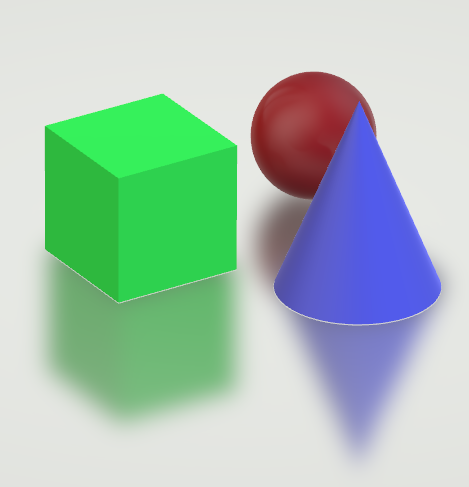
\includegraphics[scale=0.8, width=0.4\textwidth]{author/part4/figures/scene-example.png}
    \caption{Пример трехмерной сцены, визуализированной в виде двумерной проекции с определенного положения камеры}
    \label{fig:scene-example}
\end{figure}

\begin{figure}[H]
    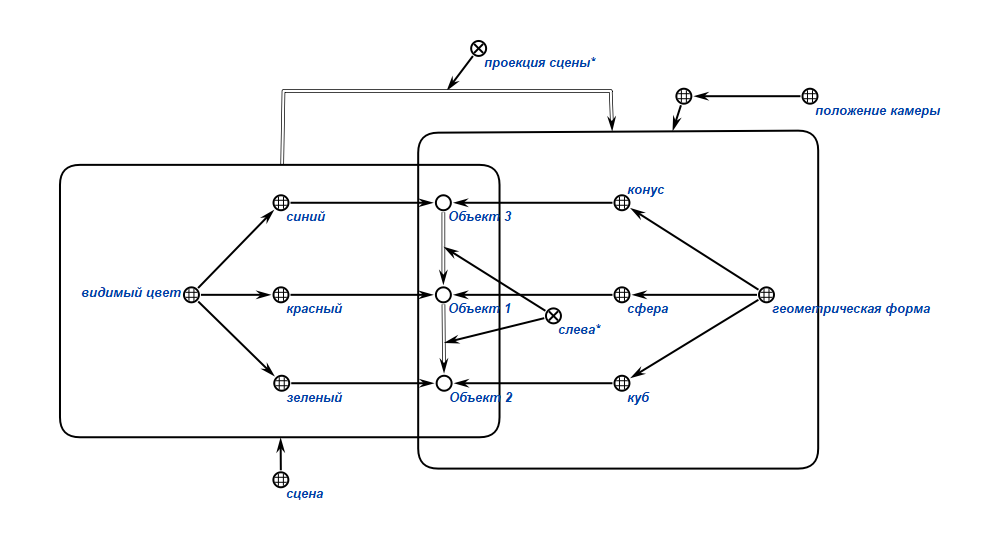
\includegraphics[scale=0.8, width=1.0\textwidth]{author/part4/figures/scene-description.png}
    \caption{Семантическое описание некоторых связей взаимного расположения объектов в сцене с положения наблюдателя}
    \label{fig:scene-description}
\end{figure}

В данном случае семантическое описание сцены в трехмерном представлении представляет собой совокупность абсолютных и относительных характеристик, что позволяет задавать семантическое наполнение различным категориям высказываний. Например, для идентификации куба приведено абсолютное описание свойства Объекта 2 ``видимый цвет'' -- ``зелёный'', но значение данного свойства может быть изменено при введении референтных отношений при таких внешних факторах как 'спектральный состав освещения' или 'наличие у наблюдателя заболевания, связанного с цветовосприятием'. 

На рисунке приведено также референтное описание относительно внешнего фактора ``положение камеры'' -- ``куб слева от конуса'', выделяющее отдельное наблюдение сцены, представляющее собой в данном случае двумерную проекцию сцены. Структура сцены в трехмерном представлении, основанная на описании присутствующих на этой сцене объектов, а также их свойств и референтных отношений относительно внешнего фактора ложится в основу семантического описания сцены в большинстве задач компьютерного зрения. Гранулярность и полнота семантического описания сцены определяется конкретной решаемой задачей. Использование такого представления открывает широкие возможности по организации человеко-машинного интерфейса, поскольку предоставляет возможность выведения необходимого контекста для определения смыслового наполнения высказываний на естественном языке. Кроме этого, такое представление может использоваться для генерации трехмерных сцен и формирования интерактивных интерфейсов взаимодействия с трехмерной средой.


\section{Трехмерное представление объектов в сцене}
\label{sec_3d_models_representation}

Как показано в предыдущем разделе системы позиционирования, распознавания и отображения объектов реального мира опираются не только на качественную составляющую описания, но и взаимное расположение объектов в пространстве или их отдельных частей. В соответствии с восприятием окружающего мира человеком трехмерное представление является наиболее информативным, хотя и не обязательным. Полученные двумерные изображения, используемые во многих задачах, являются проекциями трехмерного пространства. Поэтому для рассматриваемых в данной главе задач максимальным классом объектов исследования выбрано трехмерное представление объектов, включающее класс описаний, содержащих информацию о взаимном расположении объектов или их частей, заданных в трех координатах.

\begin{SCn}
    \scnheader{трехмерное представление объекта}
    \scnidtf{способ записи информации об объекте с сохранением его пространственных свойств в трех координатах}
    \begin{scnrelfromset}{разбиение}
        \scnitem{дискретное трехмерное представление}
        \scnidtf{трехмерное представление информации об объекте в виде дискретной совокупности трехмерных геометрических примитивов}
        \begin{scnrelfromset}{включает}
            \scnitem{воксельное представление}
            \scnidtf{представление в виде совокупности элементов, расположенных в регулярной сетке в трехмерном пространстве}
            \scnitem{облако точек}
            \scnidtf{трехмерное представление в виде неструктурированной совокупности точек}
            \scnitem{карта глубины}
            \scnidtf{двумерное изображение, на котором яркость пикселя определяет расстояние от плоскости изображения до соответствующей точки в пространстве}
        \end{scnrelfromset}
        \scnitem{поверхностное представление}
        \scnidtf{представление информации об объекте в виде совокупности поверхностей}
        \begin{scnrelfromset}{включает}
            \scnitem{аналитически задаваемая поверхность}
            \scnidtf{поверхность, заданная в трехмерном пространстве аналитически, например, уравнением}
            \scnitem{полигональная сетка}
            \scnidtf{совокупность вершин, ребер и граней, задающая некоторый многогранник в трехмерном пространстве}
            \scnitem{NURBS-поверхность}
            \scnidtf{поверхность, задаваемая с помощью совокупности неоднородных рациональных B-сплайнов через последовательность контрольных точек}
            \scnitem{поверхность разделения}
            \scnidtf{поверхность, образованная из полигональной сетки с помощью рекурсивного разделения граней этой сетки}
            \scnitem{поверхность на основе T-сплайнов}
            \scnidtf{модификация NURBS-поверхности, для которой последовательность контрольных точек может терминироваться без полного обхода всей поверхности}
        \end{scnrelfromset}
        \scnitem{специальные представления}
        \begin{scnrelfromset}{включает}
            \scnitem{видео 360}
            \scnidtf{видеопоследовательность, полученная с помощью захвата окружающего пространства во всех направлениях}
        \end{scnrelfromset}
    \end{scnrelfromset}
\end{SCn}

\begin{SCn}
    \scnheader{трехмерная модель объекта}
    \scnidtf{представление информации о конкретном объекте, записанное на основе одного из возможных трехмерных представлений}
\end{SCn}

Ниже даны определения некоторых терминов, относящихся к предметной области геометрии, стереометрии, функционального анализа и топологии, но необходимых для дополнения описания рассматриваемых видов трехмерного представления.

\begin{SCn}
    \scnheader{точка}
    \scnidtf{местоположение в пространстве, однозначно определяемое в системе координат}
\end{SCn}

\begin{SCn}
    \scnheader{геометрический примитив}
    \scnidtf{объект трехмерного пространства, который является атомарным (то есть непредставляемый в виде совокупности других объектов)}
\end{SCn}

\begin{SCn}
    \scnheader{вершина}
    \scnidtf{точка в трехмерном пространстве, задаваемая тремя координатами}
\end{SCn}

\begin{SCn}
    \scnheader{ребро}
    \scnidtf{отрезок между двумя вершинами}
\end{SCn}

\begin{SCn}
    \scnheader{грань}
    \scnidtf{замкнутая совокупность копланарных ребер}
\end{SCn}

\begin{SCn}
    \scnheader{полигон}
    \scnidtf{совокупность копланарных граней}
\end{SCn}

\begin{SCn}
    \scnheader{поверхность}
    \scnidtf{двумерное топологическое многообразие}
\end{SCn}

\begin{SCn}
    \scnheader{B-сплайн}
    \scnidtf{базисный сплайн}
    \scnidtf{сплайн-функция с наименьшим носителем для заданной степени порядка гладкости и разбиения области определения}
\end{SCn}


\section{Трехмерная реконструкция объектов окружающего мира}
\label{sec_3d_models_reconstruction}

Получить трехмерное представление на основе экспериментальных данных позволяет трехмерная реконструкция. Предметная область трехмерного представления объектов затрагивает, как само описание объекта, так и методы его получения.

\begin{SCn}
    \scnheader{трехмерная реконструкция}
    \scnidtf{задача определения истинной формы объектов в трехмерном пространстве на основании информации об этих объектах, получаемой в результате измерений, наблюдений или опытов}
\end{SCn}

Несмотря на то, что часть указанных выше задач требует дополнительных действий, все они основываются на получении трехмерного представления объекта. В соответствии с этим каждая из задач также дополнительно может быть определена как внутренним состоянием, так и описанием условий, в рамках которых она осуществляется:
\begin{textitemize}
    \item описание цели -- тип трехмерного представления, его разрешающая способность и точность,
    \item условия по возможности осуществления действий -- например, имеющееся оборудование или допустимое время выполнения,
    \item вид входных данных -- описание типа входного объекта.
\end{textitemize}

Трехмерное представление объекта или окружения, независимо от конкретного подкласса, может быть получено разными методами, в то же время конкретный метод может определять только одно представление.

\begin{SCn}
    \scnheader{методы трехмерной реконструкции}
    \begin{scnrelfromset}{включает}
        \scnitem{методы фотограмметрической реконструкции}
        \scnidtf{методы интерпретации изображений для определения трехмерной формы и положения объекта по одной или нескольким фотографиям этого объекта}
        \begin{scnrelfromset}{подразделяется по взаимному положению объекта и камеры на}
            \scnitem{мобильные системы}
            \scnitem{макрофотограмметрия}
            \scnitem{спутниковая фотограмметрия}
            \scnitem{аэрофотограмметрия}
            \scnitem{наземная фотограмметрия}
            \scnitem{ближняя фотограмметрия}
        \end{scnrelfromset}
        \begin{scnrelfromset}{подразделяется по виду входной информации на}
            \scnitem{одно изображение}
            \scnitem{стерео изображения}
            \scnitem{многокадровые}
        \end{scnrelfromset}
        \scnitem{методы томографической реконструкции}
        \begin{scnrelfromset}{включает}
            \scnitem{реконструкция на основе Фурье-проекций }
            \scnitem{алгоритм обратной проекции}
            \scnitem{алгоритм итерационной реконструкции}
            \begin{scnrelfromset}{включает}
                \scnitem{ART}
                \scnitem{SART}
                \scnitem{SAMV}
            \end{scnrelfromset}
            \scnitem{реконструкция по коническому лучу}
            \scnitem{реконструкция на основе методов глубокого обучения }
        \end{scnrelfromset}
        \scnitem{методы структурированного подсвета}
        \begin{scnrelfromset}{включает}
            \scnitem{методы на основе световых сечений}
            \scnitem{методы на основе проекций полос}
            \scnitem{методы на основе фазового сдвига}
        \end{scnrelfromset}
        \scnitem{методы по оценке отраженного сигнала}
        \begin{scnrelfromset}{включает}
            \scnitem{измерение расстояния методами оптической модуляции}
            \scnitem{импульсная модуляция}
        \end{scnrelfromset}
        \scnitem{методы оценки по фокусировке}
        \begin{scnrelfromset}{включает}
            \scnitem{методы оценки из фокусировки}
            \scnitem{методы оценки из расфокусировки }
        \end{scnrelfromset}
        \scnitem{методы на основе теоремы о Фурье-проекциях}
        \scnitem{нейросетевые модели}
    \end{scnrelfromset}
\end{SCn}

Выше представлен один из вариантов онтологического описания методов создания трехмерных представлений. Каждый из методов трехмерной реконструкции в рамках этого описания может быть определен также кроме физического принципа его разрешающей способностью, типом входных данных, размером реконструируемых объектов и т.д. Полное описание представляет собой неиерархическую онтологическую модель, строющуюся на основе базы данных ostis-системы. Для дальнейшего взаимодействия агентов с данной структурой все эти описания ставятся в соответствие некоторым характеристикам. Характеристики могут относится как к отдельному методу, так и к группе методов, например, разрешающая способность может быть общей для всего подкласса электромагнитных волновых методов. Данные характеристики должны получаться агентами из самого представления знаний динамически, что позволяет дополнять и модифицировать общую структуру.
Для удобства представления данные характеристики можно выделить в спецификацию метода, на основании которой описывается область и возможность его применения. Она дает возможность использования методов для решения конкретных прикладных задач. В рамках спецификации (и, соответственно, структуры представления методов в базе знаний) задаются:
\begin{textitemize}
    \item тип возможных входных параметров,
    \item тип выходного представления -- в данном случае соответствующее трехмерное представление;
    \item время работы;
    \item разрешающая способность метода;
    \item расстояние от объекта до камеры;
    \item тип реконструируемого объекта:
    \item композиция сцены (отдельный объект, группа объектов, окружающее пространство);
    \item тип поверхности (глянцевость, прозрачность, цветность);
    \item наличие внутренней структуры;
    \item размер объекта.
\end{textitemize}

Описанная спецификация может быть интерпретируема промежуточным отношением для каждого метода. При наличии такого описания для промежуточных этапов данный подход позволяет проводить также комбинацию методов. Например, методы радиочастотного диапазона не дают возможность построить карту глубины, но позволяют получить положение камеры в глобальной системе координат в конкретный момент времени.

\section{Системы локального позиционирования, использующиеся в задачах трехмерной реконструкции}
\label{sec_3d_models_positioning}

В основе многих систем трехмерной реконструкции лежит решение задачи локального позиционирования. Следует отметить, что в целом задача локального позиционирования является более общей, однако обычно рассматривается относительно наблюдателя, а не объекта.

\begin{SCn}
    \scnheader{система локального позиционирования}
    \scnidtf{автоматизированная система, обеспечивающая идентификацию, определение координат, отображение на плане местонахождения контролируемых объектов или их частей в пределах территории, охваченной необходимой инфраструктурой}
\end{SCn}

Характеристики систем локального позиционирования:
\begin{textitemize}
    \item точность позиционирования,
    \item достоверность позиционирования,
    \item периодичность опроса,
    \item надежность,
    \item габаритность.
\end{textitemize}

\begin{SCn}
    \scnheader{методы локального позиционирования}
    \begin{scnrelfromset}{включает}
        \scnitem{триангуляционные методы}
        \begin{scnindent}
            \scnidtf{методы, основанные на определении направления на источник сигнала}
            \scnitem{угол прихода сигнала}
            \begin{scnindent}
                \scnidtf{angle of arrival}
                \scnidtf{AoA}
                \scnidtf{направление, из которого принимается сигнал (например, радио, оптический или акустический)}
            \end{scnindent}
            \scnitem{угол вылета}
            \begin{scnindent}
                \scnidtf{angle of departure}
                \scnidtf{AoD}
                \scnidtf{направление, в котором отправляется сигнал (например, радио, оптический или акустический)}
            \end{scnindent}
        \end{scnindent}
        \scnitem{трилатерационные методы}
        \begin{scnindent}
            \scnidtf{методы, основанные на трилатерации, то есть на основе построения на местности смежных треугольников}
            \scnitem{время прибытия}
            \begin{scnindent}
                \scnidtf{time of arrival}
                \scnidtf{ToA}
                \scnidtf{абсолютный момент времени, когда радиосигнал, исходящий от передатчика, достигает удаленного приемника}
            \end{scnindent}
            \scnitem{разница во времени прибытия}
            \begin{scnindent}
                \scnidtf{time difference of arrival}
                \scnidtf{TDoA}
                \scnidtf{разница между временем прибытия сигнала до двух базовых станций}
            \end{scnindent}
            \scnitem{время полета}
            \begin{scnindent}
                \scnidtf{time of flight}
                \scnidtf{ToF}
                \scnidtf{время, затрачиваемое объектом, частицей или волной (акустической, электромагнитной и т. д.) на преодоление расстояния через среду}
            \end{scnindent}
            \scnitem{двустороннее определение дальности}
            \begin{scnindent}
                \scnidtf{two-way ranging}
                \scnidtf{TWR}
                \scnidtf{метод определения дальности, который использует две задержки, которые обычно возникают при передаче сигнала, для определения дальности между двумя станциями: задержка распространения сигнала между двумя беспроводными устройствам, задержка обработки подтверждений в беспроводном устройстве}
            \end{scnindent}
            \scnitem{симметричное двустороннее определение дальности}
            \begin{scnindent}
                \scnidtf{symmetrical double-sided two-way ranging}
                \scnidtf{SDS TWR}
                \scnidtf{метод определения дальности, который использует двустороннее определение дальности дважды: относительно базовой станции и относительно мобильного устройства}
            \end{scnindent}
        \end{scnindent}
        \scnitem{методы на основе измерения силы сигнала}
        \begin{scnindent}
            \scnidtf{received signal strength indicator}
            \scnidtf{RSSI}
            \scnidtf{индикатор уровня мощности принимаемого сигнала. Данный метод позволяет определить местоположение устройства, основываясь на уровне силы сигнала, полученного БС или наоборот}
        \end{scnindent}
        \scnitem{одометрия}
        \begin{scnindent}
            \scnidtf{использование данных о движении приводов для оценки перемещения}
            \scnitem{визуальная одометрия}
        \end{scnindent}
    \end{scnrelfromset}
\end{SCn}

\begin{SCn}
    \scnheader{физические принципы позиционирования}
    \begin{scnrelfromset}{включает}
        \scnitem{акустические}
        \begin{scnindent}
            \scnidtf{основаны на использовании ультразвуковых (высокочастотных) звуковых волн}
        \end{scnindent}
        \scnitem{радиочастотные}
        \scnitem{магнитные}
        \begin{scnindent}
            \scnidtf{магнитный трекинг основан на измерении интенсивности магнитного поля в различных направлениях. Как правило, в таких системах есть базовая станция, которая генерирует переменное или постоянное магнитное поле}
        \end{scnindent}
        \scnitem{оптические}
        \begin{scnindent}
            \scnidtf{совокупность методов позиционирования на основе данных с камер видимого или инфракрасного диапазона}
            \scnitem{с внешней камерой}
            \scnitem{с внутренней камерой}
            \begin{scnindent}
                \scnitem{визуальная одометрия}
                \begin{scnindent}
                    \scnidtf{метод оценки положения и ориентации робота или иного устройства с помощью анализа последовательности изображений, снятых установленной на нем камерой (или камерами)}
                \end{scnindent}
            \end{scnindent}
            \scnitem{лазерное позиционирование}
            \begin{scnindent}
                \scnidtf{группа методов, основанных на оценке времени прохождения лазерных импульсов определенной периодичности}
            \end{scnindent}
        \end{scnindent}
        \scnitem{инерциальные}
        \begin{scnindent}
            \scnidtf{инерциальное позиционирование основано на свойствах инерции тел. основная особенность этих методов состоит в том, что они не требуют внешних ориентиров или поступающих извне сигналов}
            \scnitem{гироскоп}
            \scnitem{акселерометр}
            \scnitem{магнитометр}
            \scnitem{барометр}
            \scnitem{гибридные}
        \end{scnindent}
    \end{scnrelfromset}
\end{SCn}

Описание и дальнейшее проектирование различных систем локального позиционирования вызывает необходимость использования и других разделов базы знаний ostis-системы. 

\section{Базовые понятия компьютерного зрения в задаче трехмерной реконструкции}
\label{sec_3d_models_computervision}

\subsection{Оптические системы компьютерного зрения}

Компьютерное (техническое) зрение как отдельная область исследований начала формироваться еще в 1960-х г. как попытка имитировать зрительную систему человека в робототехнике. Данное направление изначально основывалось на достижениях в области цифровой обработки изображений, однако в дальнейшем расширило перечень рассматриваемых задач в том числе засчет попытки извлечения трехмерной структуры изображений с целью более полного понимания сцены. Понимание в этом контексте означает преобразование визуальных образов в описания мира, которые могут взаимодействовать с другими процессами и вызывать соответствующие действия. Считается, что в область компьютерного зрения входят задачи распознавания образов, наблюдения, роботизированного управления, сегментации и интерпретации медицинских изображений, автоматического осмотра и сборки в заводских условиях, распознавания отпечатков пальцев и лиц, интерпретации жестов и многие другие (см. \scncite{Davies2021}).

\begin{SCn}
    \scnheader{компьютерное зрение}
    \scnidtf{техническое зрение}
    \scnidtf{междисциплинарная предметная область, описывающая совокупность технологий, методов и алгоритмов регистрации, обработки, анализа и получения символьного описания потоков данных с помощью различных источников визуальной информации, включая камеры видимого и инфракрасного спектра, трехмерные датчики и другие устройства визуализации, такие как компьютерные и магнитно-резонансные томографы.}
\end{SCn}

В области трехмерной реконструкции используются системы, регистрирующие излучение в различных диапазонах длин волн -- от рентгеновского (рентгеновский сканер) до радиоволнового (электромагнитная катушка). Наиболее распространенным подходом для анализа является использование излучения в видимом диапазоне (380 нм -- 720 нм), регистрируемого оптической системой компьютерного зрения, например, камерой (фотоаппаратом). 

\begin{SCn}
    \scnheader{оптическая система компьютерного зрения}
    \scnidtf{совокупность оптических элементов, обеспечивающая регистрацию электромагнитного поля видимого, ультразвукового и инфракрасного диапазона с целью дальнейшей обработки и получения количественного и символьного описания информации.}
\end{SCn}

Одним из наиболее распространенных видов оптической системы для регистрации информации об объекте является цифровая камера. При использовании цифровой камеры формой представления полученных данных является снимок, который может быть представлен в виде растрового изображения. При этом в контексте конкретной рассматриваемой задачи важными могут являться не только параметры полученного изображения, но и фиксация условий проведения съемки и параметров оптической системы.  

Изображение является двумерной проекцией исходного трехмерного пространства. Трехмерную модель рассматриваемого объекта по нескольким снимкам или видеоряду можно получить на основе восстановления параметров проекций, связанных с каждым из снимков, и выстраиванием этих проекций в одном трехмерном пространстве. При наличии пересекающихся лучей, направленных в одну и ту же точку реального объекта, по проекциям можно восстановить параметры объекта и сцены в связанной с этим пространством системе координат. По схожему принципу устроена зрительная система человека, основанная на анализе разницы между изображениями, получаемыми левым и правым глазом, а также последовательно полученными изображениями на сетчатке одного глаза в небольшом временном диапазоне.

\begin{SCn}
    \scnheader{проекция}
    \scnidtf{отображение точек, фигур, векторов пространства любой размерности на его подпространство любой размерности}
\end{SCn}

\begin{SCn}
    \scnheader{бинокулярное зрение}
    \scnidtf{способность одновременно чётко видеть изображение предмета обоими глазами; в этом случае человек видит одно изображение предмета, на который смотрит}
\end{SCn}

\begin{SCn}
    \scnheader{стереоскопическое зрение}
    \scnidtf{вид зрения, при котором возможно восприятие формы, размеров и расстояния до предмета, благодаря восприятию двух изображений, полученных в пределах бесконечно малого промежутка времени при разных параметрах внешнего ориентирования оптической системы в пространстве}
\end{SCn}

Для описания преобразования между объектами в исходном трехмерном пространстве и их проекцией используется модель проекции. Модель проекции при использовании в системах трехмерной реконструкции описывает ход световых лучей в оптической системе и относится к области изучения эпиполярной геометрии. Наиболее известной, использующейся в геометрии является модель ортогональной проекции. Но для работы с оптическими системами больше подходит модель центральной проекции, которая описывает ход лучей в камере-обскуре.  Оптическую систему съемки можно считать аналогичной камере-обскуре, если она содержит симметричную систему линз и не вносит криволинейных искажений, т.е. все прямые исходной трехмерной сцены остаются прямыми и не искривляются после проекции. В общем случае модель проекции может учитывать различные особенности оптической системы или среды получения изображения. Например, в работе \scncite{Halavataya2019} предлагается модель широкоугольной сферической проекции, учитывающая дисторсионные искажения, вызываемые широкоугольной камерой. Использование корректной модели проекции напрямую влияет на качество реконструируемых трехмерных сцен и объектов.

\begin{SCn}
    \scnheader{эпиполярная геометрия}
    \scnidtf{один из подразделов оптики, который занимается геометрической интерпретацией формирования двумерных изображений по трехмерной сцене. Чаще всего в этом контексте рассматривается задача геометрических преобразований лучей света, которые отражаются от наблюдаемой трехмерной сцены, улавливаются некоторой оптической системой или объективом и проецируются на фоточувствительную двумерную поверхность (например, плёнку или цифровую матрицу) для формирования изображения}
\end{SCn}

\begin{SCn}
    \scnheader{модель проекции}
    \scnidtf{математическая модель, в соответствии с которой осуществляется построение проекции}
    \begin{scnrelfromset}{включает}
        \scnitem{параллельная проекция}
        \scnidtf{вид проекции, при котором проецирующиеся лучи строятся параллельными друг другу}
        \begin{scnindent}    
            \scnitem{ортогональная проекция}
            \scnidtf{вид параллельной проекции, в которой проецирующие лучи строятся перпендикулярно некоторой заданной плоскости, например, плоскости изображения}
        \end{scnindent}
        \scnitem{центральная проекция}
        \scnidtf{вид проекции, при котором все прямые, построенные на проецирующихся лучах, пересекаются в одной точке, называемой центром проекции. Параллельная проекция может считаться предельным случаем центральной проекции с центром проекции, удаленным на бескнечное расстояние}
    \end{scnrelfromset}
\end{SCn}

Для полного задания модели проекции вводятся параметры, называемые параметрами ориентирования, однозначно характеризующие положение снимка относительно некоторой глобальной системы координат. Выделяют параметры внутреннего и внешнего ориентирования. Параметры внутреннего ориентирования задают относительное положение точки фотографирования и самого снимка. В модели центральной проекции к параметрам внутреннего ориентирования относятся 3 величины: двумерные координаты главной точки снимка $(x_0,y_0)$ и фокусное расстояние $f$. К параметрам внешнего ориентирования относят 6 величин, задающих связь проецирующих лучей в момент съемки с глобальной системой координат: координаты точки положения камеры $(x_C,y_C,z_C)$, два угла, определяющие положение главного луча камеры $(\omega,\varphi)$ и угол поворота снимка $\beta$. Для перехода в новое пространство необходимо осуществить пространственное преобразование между системами координат. Для этого используется преобразование Гельмерта, зависящее от 7 параметров: координаты начала системы координат снимка xyz в глобальной координатной системе OXYZ $(X_0,Y_0,Z_0)$, три угла поворота $(\omega,\varphi, \beta)$ относительно осей $X$,$Y$,$Z$ и коэффициент масштаба $m$. На основании данных углов можно построить матрицу поворота, задающую преобразование координат из одной системы в другую при последовательном повороте вокруг каждой из осей.

\begin{SCn}
    \scnheader{параметры ориентирования модели центральной проекции}
    \scnidtf{параметры, задающие связь координат объекта на изображении и в трехмерном пространстве при условии, что ход лучей и, соответственно, формирование изображения в оптической системе описывается центральной проекцией }
    \begin{scnrelfromset}{включает}
        \scnitem{параметры внутреннего ориентирования}
        \begin{scnrelfromset}{включает}
            \scnitem{фокусное расстояние}
            \scnitem{координаты главной точки снимка ($x_0$, $y_0$)}
        \end{scnrelfromset}
        \scnitem{параметры внешнего ориентирования}
        \begin{scnrelfromset}{включает}
            \scnitem{координаты точки положения камеры ($x_C$, $y_C$, $z_C$)}
            \scnitem{углы, определяющие положение главного луча камеры $(\omega,\varphi)$}
            \scnitem{угол поворота снимка $\beta$}
        \end{scnrelfromset}
    \end{scnrelfromset}
\end{SCn}

\begin{SCn}
    \scnheader{калибровка камеры}
    \scnidtf{задача получения внутренних и внешних параметров камеры по имеющимся фотографиям или видео, отснятыми ею}
\end{SCn}

Калибровка камеры часто используется на начальном этапе решения многих задач компьютерного зрения и, в особенности, задач, связанных с дополненной реальностью. Кроме того, калибровка камеры может использоваться для исправления искажений, вызванных оптической системой съемки, например, дисторсии.

\begin{SCn}
    \scnheader{оптическая аберрация}
    \scnidtf{отклонение от идеальной модели формирования изображения в оптической системе}
\end{SCn}

\begin{SCn}
    \scnheader{дисторсия}
    \scnidtf{аберрация оптических систем, при которой коэффициент линейного увеличения изменяется по мере удаления отображаемых предметов от оптической оси}
    \begin{scnrelfromset}{включает}
        \scnitem{радиальная дисторсия}
        \scnidtf{дисторсия, вызванная сферической поверхностью линз оптической системы}
        \scnitem{тангенциальная дисторсия}
        \scnidtf{дисторсия, вызванная неперпендикулярностью главной оптической оси и плоскости изображения и прохождением главной оптической оси не через центр снимка}
    \end{scnrelfromset}
\end{SCn}

\subsection{Локальные признаки изображений}

Одним из первых этапов трехмерной реконструкции по изображениям, полученным с различных ракурсов, является нахождение всевозможных комбинаций соответствующих точек на изображениях, которые являются одной и той же точкой исходной сцены. Традиционно для решения этой задачи используются алгоритмы для работы с локальными признаками изображения.

\begin{SCn}
    \scnheader{локальный признак изображения}
    \scnidtf{некоторое подмножество точек изображения, пространственные окрестности которых определённым образом характеризуют изображение целиком или присутствующие на нём объекты}
    \begin{scnrelfromset}{включает}
        \scnitem{ключевая точка}
    \end{scnrelfromset}
\end{SCn}

Основной сложностью при реализации и работе с алгоритмами нахождения локальных признаков является тот факт, что универсального или однозначно точного определения того, что именно является локальным признаком, не существует. Конкретное определение локального признака в произвольной точке произвольного изображения зависит от вида используемого алгоритма и решаемой задачи. К основным концепциям, на основании которых принимается решение о наличии в точке локального признака, в различных исследованиях относят модуль и направление градиента, определяемые по разностной схеме значения лапласиана или гессиана в окрестности точки, собственные значения и векторы и т.п. В работе {\scncite{Krig2016}} приводится таксономия атрибутов описательных характеристик локальных признаков для их более высокоуровневого анализа. Алгоритмы детектирования локальных признаков на изображении, как правило, являются входной точкой для последующей обработки другими методами. Методы глубкого обучения, такие как сверточные нейронные сети, также основаны на выделении низкоуровневневых локальных признаков изображения с помощью операции свертки.

В задачах трехмерной реконструкции основной интерес представляет не само нахождения локальных признаков изображения, а их сопоставление между несколькими кадрами для нахождения смещения объектов. Зная параметры оптической системы компьютерного зрения в момент получения каждого снимка и сопоставив смещение объектов на отдельных изображениях, можно получить расстояние между объектами в глобальной системе координат. Поэтому базовой задачей является построение карты диспаратности.

\begin{SCn}
    \scnheader{диспарантность}
    \scnidtf{различие взаимного положения двух точек, отображаемых на двух изображениях и соответствующих одной точке пространства}
\end{SCn}

\begin{SCn}
    \scnheader{карта диспарантности}
    \scnidtf{набор значений, соответстветствующих пикселям исходного изображения и отображающих смещение каждого исходного пикселя относительного его положения на другом изображении. Чаще всего отображается также в виде изображения, при этом значение яркости пикселей отражает величину смещения}
\end{SCn}

Карты диспарантности могут быть получены различными методами, основанными как на статистических характеристиках отдельных областей изображений, так и на нахождении ключевых точек и сопоставлении их на основе некоторого описания окрестности (то есть значения, полученного с помощью алгоритма дескриптора). Во втором случае карта диспарантности может быть построена не для всего изображения, а только для подмножества пикселей, соответствующих ключевым точкам. Данный подход является одним из основных этапов методов фотограмметрической реконструкции, включающим нахождение всевозможных комбинаций соответствующих точек на изображениях проекций, которые относятся к одной и той же точке исходной сцены.

\begin{SCn}
    \scnheader{методы построения карты диспарантности}
    \begin{scnrelfromset}{включает}
        \scnitem{вычисление суммы абсолютных разностей для небольших окрестностей изображения}
        \scnitem{вычисление суммы квадратов разностей для небольших окрестностей изображения}
        \scnitem{вычисление нормализованной кросскорреляции для небольших окрестностей изображений}
        \scnitem{нейросетевые алгоритмы для вычисления карты диспарантности}
        \scnitem{детекторы и дескрипторы ключевых точек}
        \begin{scnindent}
            \scnitem{детекторы}
            \begin{scnindent}
                \scnidtf{алгоритмы, которые по входному изображению генерируют набор ключевых точек}
                \scnitem{эмпирические детекторы}
                \begin{scnindent}
                    \scnidtf{алгоритмы поиска ключевых точек, которые основаны на некоторых интуитивных представлениях, практическом опыте и результатах тестирования}
                    \scnitem{FAST \scncite{Rosten2006}}
                    \scnitem{детектор Харриса \scncite{Harris1988}}
                    \scnitem{Susan \scncite{Smith1997}}
                \end{scnindent}
                \scnitem{статистические детекторы}
                \begin{scnindent}
                    \scnidtf{алгоритмы поиска ключевых точек, которые основаны на сравнении статистических характеристик точки или её окрестности с некоторыми заранее известными}
                    \scnitem{SIFT \scncite{Lowe2004}}
                    \scnitem{AGAST \scncite{Mair2010}}
                \end{scnindent}
                \scnitem{детекторы на основе машинного обучения}
                \begin{scnindent}
                    \scnidtf{алгоритмы поиска ключевых точек, которые основаны, как правило, на существующих эмпирических или статистических детекторах, но использующие оптимизацию некоторых варьируемых параметров детектирования методами машинного обучения}
                    \scnitem{FAST-ER \scncite{Rosten2010}}
                    \scnitem{TILDE \scncite{Verdie2015}}
                \end{scnindent}
            \end{scnindent}
            \scnitem{дескрипторы}
            \begin{scnindent}
                \scnidtf{алгоритмы, которые по входному изображению и набору координат точек на них, генерируют вектор признаков, описывающий эти точки в некотором метрическом пространстве}
                \scnitem{гистограммные дескрипторы}
                \begin{scnindent}
                    \scnidtf{алгоритмы, строящие вектор представления для описания ключевой точки на основании гистограммы некоторой статистики, которую можно вычислить по её окрестности. Вектора описаний гистограммных дескрипторов обычно имеют размерность не менее 128, значения отдельных элементов являются вещественными числами, так как гистограмма, как правило, нормализуется}
                    \scnitem{SIFT \scncite{Lowe2004}}
                    \scnitem{SURF \scncite{Bay2008}}
                \end{scnindent}
                \scnitem{бинарные дескрипторы}
                \begin{scnindent}
                    \scnidtf{алгоритмы, разработанные с целью ускорения сопоставления векторов описаний точек и строящие вектор представления для описания ключевой точки, состоящий из элементов булева множества}
                    \scnitem{BRIEF \scncite{Calonder2010}}
                    \scnitem{ORB \scncite{Rublee2011}}
                    \scnitem{BRISK \scncite{Leutenegger2011}}
                \end{scnindent}
            \end{scnindent}
        \end{scnindent}
        \scnitem{методы оптического потока}
        \begin{scnindent}
            \scnidtf{методы отображения видимого движения объектов, поверхностей или краев сцены, получаемого в результате относительного перемещения наблюдателя и объектов сцены}
            \scnitem{фазовая корреляция}
            \begin{scnindent}
                \scnidtf{методы оптического потока, основанные на инверсии нормализованного перекрестного спектра}
            \end{scnindent}
            \scnitem{блочные методы}
            \begin{scnindent}
                \scnidtf{методы оптического потока, основанные на минимизации суммы квадратов или суммы модулей разностей}
            \end{scnindent}
            \scnitem{дифференциальные методы оценки оптического потока, основанные на частных производных сигнала}
            \begin{scnindent}
                \scnitem{алгоритм Лукаса-Канаде \scncite{Lucas1981}}
                \scnitem{Horn–Schunck \scncite{Horn1981}}
                \begin{scnindent}
                    \scnidtf{алгоритмы, основанные на минимизации функционала, описывающего отклонение от предположения о постоянстве яркости и гладкости получаемого векторного поля}
                \end{scnindent}
                \scnitem{общие вариационные методы}
                \begin{scnindent}
                    \scnidtf{методы, основанные на модификации метода Horn-Schunck, но использующие другие ограничения на данные и другие ограничения на гладкость}
                \end{scnindent}
            \end{scnindent}
            \scnitem{дискретные методы оптимизации}
            \begin{scnindent}
                \scnidtf{методы, основанные на квантовании поискового пространства и присвоении каждому пикселю изображения метки таким образом, чтобы расстояние между последовательными кадрами было минимальным}
            \end{scnindent}
        \end{scnindent}
    \end{scnrelfromset}
\end{SCn}

Количество и распределение выделенных локальных признаков изображения влияет на возможность не только проведения трехмерной реконструкции, но и на качество результатов других задач компьютерного зрения. При этом как не существует точного определения, что должен представлять локальный признак изображения, так и не существует универсального алгоритма, позволяющего работать с любым видом изображений. В работе \scncite{Halavataya2020} приведены примеры параметров изображения, на основании которых могут подбираться соответствующие параметры алгоритмов детекторов и дескрипторов ключевых точек. Данные параметры также могут быть описаны в рамках базы знаний ostis, что позволит построить адаптивную систему подбора алгоритма выделения локальных признаков в связанных задачах компьютерного зрения.

\section{Онтология действий, выполняемых в предметной области трехмерной реконструкции}
\label{sec_3d_models_actions}

На верхнем уровне любой метод трехмерной реконструкции может быть представлен в виде процедурного знания, например, в виде последовательности этапов, в соответствии с которыми входные данные для трехмерной реконструкции преобразовываются в итоговое трехмерное представление.

Общая черта многих методов трехмерной реконструкции -- использование промежуточного (или конечного) представления об объектах окружающего мира в трех координатах. Другими словами, метод трехмерной реконструкции можно представить в виде последовательности действий по формированию набора элементов, характеризующихся координатами в общем трехмерном пространстве, которые в дальнейшем, при необходимости, могут быть достроены до поверхностей, скомбинированы с двумерными представлениями и т.д. для формирования нужного выходного представления:

\begin{equation}
    r:I{m(R^3)}\rightarrow O
\end{equation}

где I -- входные данные, $R^3$ -- общее трехмерное декартово пространство, $m(R^3)$ -- описание элемента в системе координат общего трехмерного пространства, $O$ -- выходное трехмерное представление. Чаще всего в качестве элементов промежуточного представления выступают отдельные точки трехмерного пространства -- в этом случае такое представление называют облаком точек.

В качестве элементов могут также выступать отрезки кривых, аналитически задаваемые поверхности, полигоны и другие виды объектов.

В качестве источников данных о трехмерных координатах для промежуточного представления могут выступать:
\begin{textitemize}
    \item Непосредственно абсолютные значения трехмерных координат точек, т.е. в этом случае входные данные $I$ представляют собой набор точек ${R^3}$. Это характерно для всех методов, которые позволяют строить карту глубины сцены, т.к. представление в виде карты глубины с известными координатами положения наблюдателя и фокусного расстояния карты позволяет определить трехмерные координаты любой точки на ней.
    \item Данные, по которым с помощью некоторой дополнительной обработки могут быть получены значения трехмерных координат отдельных точек. Такие представления, как правило, намного более распространены и просты в получении.
\end{textitemize}

Следует отметить, что различные источники данных при формирования промежуточного представления могут использоваться совместно, при наличии у каждого из источников некоторой привязки к общей системе координат.

Как для пшолучения промежуточного трехмерного представления, так и для формирования на его основе итогового представления могут использоваться различные методы и алгоритмы, структура и взаимосвязь которых итоговую последовательность действе по выполнению трехмерной реконструции объекта или сцены.


\subsection{Действия по формированию промежуточного трехмерного представления}

Многие методы дистанционного зондирования полагаются на наличие априорной информации о трехмерных координатах исследуемого объекта, по которой можно построить облако точек для промежуточного трехмерного представления. К таким относятся методы, которые позволяют оценивать расстояние от измерительного прибора до объекта. Тем не менее, использование этих методов требует более сложного оборудования, применение которого может быть затруднено в некоторых сценариях.

В этой связи, в качестве отдельной категории методов исследования можно выделить группу методов формирования промежуточного представления в виде облака точек по более традиционным видам информации. К таким относятся методы генерации по одному изображению, стереопаре, набору изображений или по видеоряду, в которых также может использоваться информация об оптической системе камеры, которая была использована для получения изображения.

Таким образом можно выделить следующие виды входных данных:
\begin{textitemize}
    \item Статическое изображение или набор статических изображений;
    \item Видеоряд (набор статических изображений с временной меткой);
    \item Стереопара (2 статических изображения с параметрами оптической системы) или набор стереопар;
    \item Стерео-видеоряд (набор стереопар с временной меткой).
    \item Информация об оптической системе камеры.
\end{textitemize}

В качестве выходного представления в данном случае выступает разреженное облако точек трехмерного пространства, с привязкой каждой из точек этого пространства к одной или нескольким точкам исходных входных изображений.

Формирование разреженного облака точек включает в себя следующие этапы, для каждого из которых могут быть определены указанные параметры:
\begin{textitemize}
    \item Предобработка
    \item Детектирование ключевых точек
    \begin{textitemize}
        \item алгоритм-детектор
    \end{textitemize}
    \item Сопоставление ключевых точек
    \begin{textitemize}
        \item алгоритм-дескриптор или алгоритм оптического потока
        \item прореживание
    \end{textitemize}
    \item Оценка положений камеры
    \begin{textitemize}
        \item  модель проекции
        \item алгоритм оценки связок
    \end{textitemize}
    \item Постобработка
\end{textitemize}

Детектирование и сопоставление ключевых точек позволяет определить точки, принадлежащие одному и тому же объекту исследуемого трехмерного пространства, при наличии достаточного количества изображений. На этапе оценки положения камеры используется математическая модель проекции, задающая взаимосвязь между двумерными координатами точки на изображении и соответствующими ей трехмерными координатами в пространстве моделирования; на этом же этапе может осуществляться эмпирическая оценка глубины, например, при помощи нейросетевых методов. Каждое соответствие, описанное математически с помощью модели проекции, в дальнейшем используется в алгоритме оценки связок для того, чтобы восстановить в трехмерном пространстве положения камеры для каждого из исследуемых изображений, а также определить расстояния от камер до точек, исходя из некоторого критерия минимизации ошибки обратной проекции.

Например, классический метод трехмерной реконструкции Structure from Motion по нескольким
входным изображениям в рамках представленного конвейера можно описать следующими характеристиками:
\begin{textitemize}
    \item Предобработка -- преобразование к оттенкам серого;
    \item Алгоритм-детектор -- SIFT, SURF, FAST;
    \item Алгоритм-дескриптор -- SIFT, SURF, ORB;
    \item Прореживание -- RANSAC;
    \item Модель проекции -- центральная проекция;
    \item Алгоритм оценки связок -- глобальный метод связок с оптимизацией методом Левенберга-Марквардта.
\end{textitemize}
В качестве ещё одного примера рассмотрим метод одновременной локализации и построения карты ORB-SLAM, использующий в качестве входного представления видеоряд:
\begin{textitemize}
    \item Предобработка -- прореживание кадров;
    \item Алгоритм-детектор -- FAST;
    \item Алгоритм-дескриптор -- ORB + метод оптического потока Лукаса-Канаде;
    \item Прореживание -- RANSAC, прореживание по инвариантам движения;
    \item Модель проекции -- центральная проекция;
    \item Алгоритм оценки связок -- инкрементальный метод связок с фиксированным положением камеры и фиксированным положением ключевых точек между кадрами, метод построения карты по движению;
    \item Постобработка -- уточнение траектории и детектирование петель.
\end{textitemize}

Онтологическое описание представленной последовательности действий, а также пример конкретного алгоритма, реализованного по этой последовательности действий в рамках ostis-системы, представлены на рисунках \textit{\nameref{fig:reconstruction}} и \textit{\nameref{fig:reconstruction-example}}.

\begin{figure}[H]
    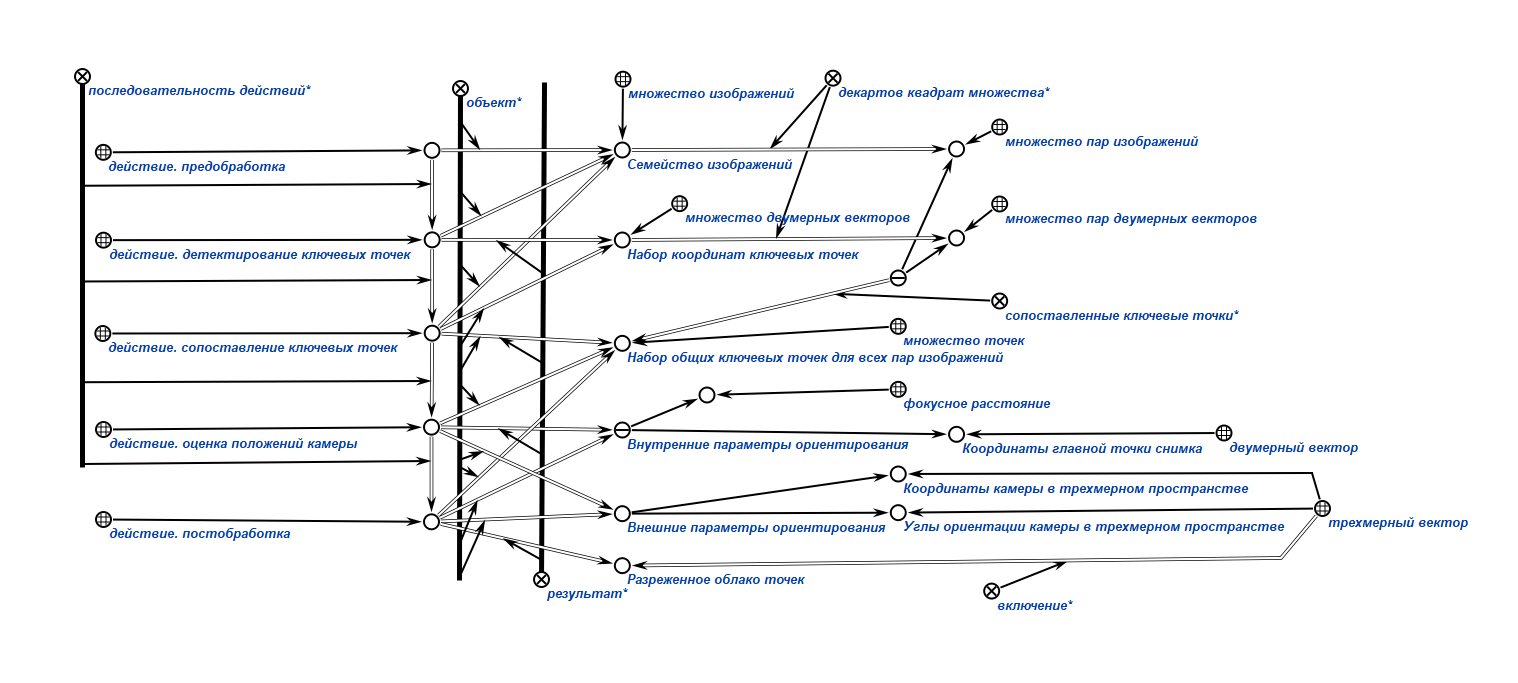
\includegraphics[scale=0.8, width=1.0\textwidth]{author/part4/figures/reconstruction.png}
    \caption{Онтологическое описание последовательности действий по построению промежуточного трехмерного представления в виде разреженного облака точек}
    \label{fig:reconstruction}
\end{figure}

\begin{figure}[H]
    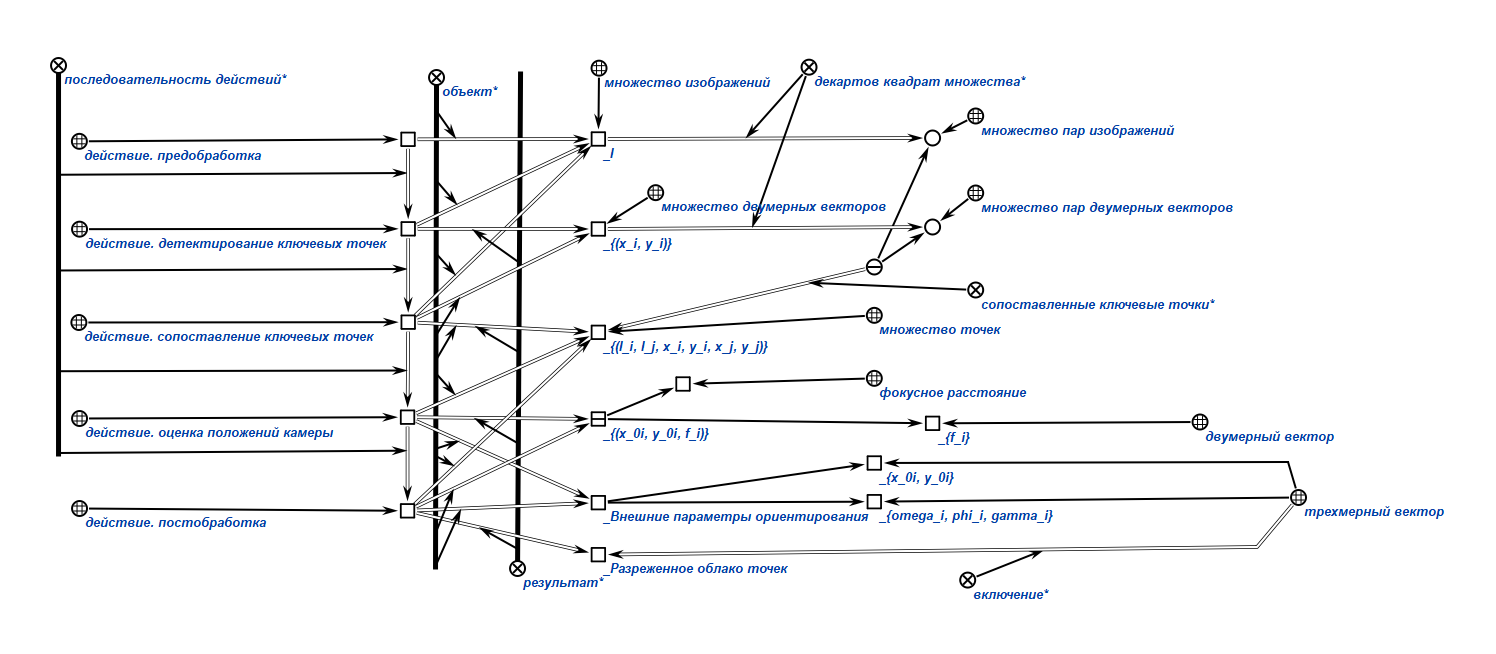
\includegraphics[scale=0.8, width=1.0\textwidth]{author/part4/figures/reconstruction-example.png}
    \caption{Пример алгоритма построения разреженного облака точек на основе представленного описания}
    \label{fig:reconstruction-example}
\end{figure}

Поскольку каждый из предложенных этапов описан в виде функционального отображения, предполагается добавление, удаление или модификацию этапов при обработке, если соблюдается соответствие типов входных и выходных представлений в контексте решаемой задачи.

\subsection{Действия по формированию итогового трехмерного представления}

В некоторых задачах разреженное облако точек в трехмерном пространстве может выступать достаточным представлением, и может считаться итогом работы алгоритма трехмерной реконструкции. Также достаточно популярным является представление в виде уплотненного цветного облака точек.

Тем не менее, во многих задачах такого представления недостаточно, поэтому можно выделить класс действий при формировании более сложного трехмерного представления, в зависимости от типа требуемого выходного представления. В качестве входного представления для этого этапа выступает разреженное облако точек, а также дополнительная информация о связи конкретных точек облака с исходными представлениями.

Описание методов формирования итогового трехмерного представления можно представить в виде совокупностей следующих этапов, с соответствующими параметрами:
\begin{textitemize}
    \item Уплотнение облака точек
    \begin{textitemize}
        \item алгоритм уплотнения
        \item связь с исходными данными
    \end{textitemize}
    \item Формирование поверхностей
    \begin{textitemize}
        \item тип поверхности
        \item алгоритм формирования поверхностей
    \end{textitemize}
    \item Уточнение поверхностей
    \begin{textitemize}
        \item алгоритм уточнения поверхностей
        \item связь с исходными данными
    \end{textitemize}
    \item Текстурирование поверхностей
    \begin{textitemize}
        \item метод текстурирования
        \item связь с исходными данными
        \item разрешение конфликтов
    \end{textitemize}
\end{textitemize}

На этапе уплотнения облака точек информация о связи трехмерных координат точек разреженного облака с исходными данными используется для переноса дополнительных точек напрямую из исходного представления в трехмерную модель. Далее путём анализа полученного плотного облака точек и исходных данных формируется грубая оценка итоговой трехмерной поверхности в виде некоторого трехмерного примитива, как правило, путём формирования полигональной сетки объединением ближайших точек в треугольники. На этапе уточнения поверхностей может происходить сглаживание, прореживание и объединение примитивов, полученных на предыдущем этапе, на основании некоторой информации из исходных данных. Наконец, на этапе текстурирования исходное представление переносится в построенную трехмерную модель, чтобы обеспечить её реалистичность; также на этом этапе происходит разрешение конфликтов для выбора корректной стратегии текстурирования в условиях наличия нескольких равноправных источников информации о текстуре.

Например, алгоритм реконструкции поверхностей, предложенный в рамках наиболее популярной на сегодняшний день реализации метода связок можно описать в виде следующего набора параметров:
\begin{textitemize}
    \item алгоритм уплотнения -- перенос окрестностей ключевых точек
    \item тип поверхностей -- полигональные с прямоугольными полигонами
    \item алгоритм формирования поверхностей -- оценка переносов камеры с помощью триангуляции Делоне, оценка планарных переносов камеры, интерполяция между положениями камеры, ручная подстройка
    \item алгоритм уточнения поверхностей -- отсутствует
    \item метод текстурирования -- прямой перенос с исходных изображений
    \item метод разрешения конфликтов текстурирования -- альфа-смешение пропорционально расстоянию до точки.
\end{textitemize}

\subsection{Действия по подбору и генерации алгоритма}

Подробное описание структуры методов не является достаточным для непосредственного выполнения трехмерной реконструкции по некоторому алгоритму. Поскольку для каждого из этапов итогового конвейера существует большое множество реализаций, возникает также задача оптимального выбора из набора реализаций каждого из этапов для наиболее эффективного решения поставленной задачи.

Как для выбора этапов алгоритма трехмерной реконструкции, так и для его непосредственной реализации может использоваться агентно-ориентированный подход к обработке информации. Коммуникация агентов осуществляется на основе обращения к общему представлению в базе знаний, по которой генерируется ряд вопросов, специфицирующих дальнейшие действия.

В качестве основных вопросов, на основании которых может осуществляться генерация алгоритма, можно выделить следующие:
\begin{textitemize}
    \item Какие входные данные будут использоваться для реконструкции?
    \begin{textitemize}
        \item Можно ли по входным данным определить расстояние до точки в трехмерном пространстве, или непосредственно её трехмерные координаты?
        \item В качестве данных будут использованы изображения?
        \begin{textitemize}
            \item Известны ли оптические параметры камеры?
            \item Известны ли положения или ориентации камеры в пространстве для каждого изображения?
            \item Является ли набор изображений непрерывным видеорядом с известной частотой кадров?
        \end{textitemize}
        \item При наличии нескольких источников входных данных, имеется ли информация о привязке описываемых ими данных к общей системе координат?
    \end{textitemize}
    \item Какой тип трехмерной модели должен быть сформирован по этим данным?
    \begin{textitemize}
        \item Требуется ли реконструкция трехмерных поверхностей?
        \begin{textitemize}
            \item Могут ли исходные данные использоваться для формирования текстур поверхностей?
        \end{textitemize}
    \end{textitemize}
\end{textitemize}

На основе рассмотренного подхода может осуществляться как подбор метода, удовлетворяющего требованиям задачи, так и подбор отдельных этапов алгоритма, например, выбор наиболее оптимального алгоритма детектирования и описания ключевых точек.
Кроме этого, может осуществляться комбинация 3D-представлений, полученных разными методами (см. \scncite{Halavataya2022a}).

\section*{Заключение к Главе~\ref{chapter_3D_models}}

В главе рассмотрено онтологическое описание предметной области трехмерной реконструкции объектов и действий по их обработке в базах знаний на основе технологии OSTIS. Описание представлено в виде доменной области самих представлений, методов их получения и соответствующих действий по их обработке.

Преимуществами использования технологии OSTIS для рассмотренных задач являются:

\begin{textitemize}
    \item Введение общей системы понятий и описаний методов в унифицированном и согласованном виде.
    \item Возможность конвергенции предметной области трехмерной реконструкции с предметной областью формирования трехмерных сцен и окружений и смежными областями.
    \item Упрощение разработки прикладных систем, использующих методы трехмерной реконструкции.
    \item Возможность построения комплексной технологии проектирования с использованием интеллектуальных агентов, потребляющих предложенное описание.
    \item Возможность создания средств интеграции отдельных компонентов, этапов различных методов и полученных внутренних представлений.
\end{textitemize}

С помощью предложенного подхода становится возможным создавать интеллектуальные системы, которые могут получать и оперировать трехмерным представлением для дальнейшей обработки в прикладных задачах.
